This study quantifies the effect of the scintillating fiber diameter on the detection of cosmic ray events. The energy deposited in the scintillating fiber by a cosmic ray event is proportional to the active volume crossed, which is larger for $2~\mm$ fibers. Therefore, the cosmic ray signal obtained for a measured cosmic event will be larger for a detector based on $2~\mm$ diameter. The objective of this study is to find the design with which a lower background is obtained in the region of interest of tritium detection, ROI (up to $18~\keV$).

The distribution of energy deposited in scintillating fibers by cosmic ray events are shown in figure \ref{fig:DiameterComparison} for both cases, $1~\mm$ and $2~\mm$ fibers.

\begin{figure}[hbtp]
\centering
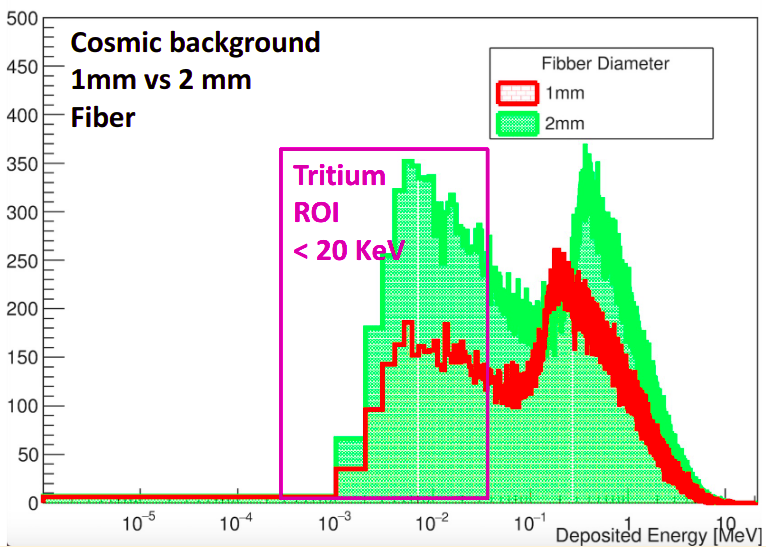
\includegraphics[scale=0.4]{Figures/8SimulationsResults/81TRITIUMDesign/814Diameter/ComparisonDiameter.png}
\caption{Comparison of the energy deposition of cosmic ray events in scintillating fibers of $1~\mm$ and $2~\mm$ in diameter.\label{fig:DiameterComparison}}
\end{figure}

As can be seen in the figure, a smaller background is measured for fiber diameters of $1~\mm$, which reduces the low detection level LDL of the detector. There are other reasons that favor the use of $2~\mm$ fibers, such us their greater resistance and an improvement to the passage of water through them, so a experimental test is needed to choose the best design.


%%A study was carried out to quantify the effect of the the scintillating fibers diameter on tritium measurement. It doesn't have sense to simulate a tritiated water source since the tritium detection efficiency is proporitonal to the active area. However it is insteresting to measure the the background of the TRITIUM prototype due to the cosmic rays since 